\section{Modeling Solar Modules}\label{sec:modeling_solar_modules}

After modeling the solar cell, the next layer up in the abstraction chain is
modeling a solar module. A solar module, in a typical configuration, may consist
of several solar cells in series, also called a `string'. For the \ac{LHRs}
vehicle, we place many modules in series with each other before terminating at
our variable load, a \acf{MPPT}. In our configuration, for each module, we place
a `bypass diode' in antiparallel to each module. This is used to provide an
alternative path of current to flow in the event that a solar module is
insufficient for driving the current. This could happen if a single (or several)
solar cell(s) in the module is (are) broken, or shaded, or some combination of
the two.

In this section, we'll focus on the conditions that cause issues with solar
modules, in particular, cell mismatch. We'll look at how cells with differing
operating conditions in series can drag down the efficiency of the module, and
we'll incorporate the bypass diode into the model and investigate the
conditions in which it activates and to what degree it activates.

\subsection{Modeling Photovoltaic Strings}\label{subsec:solar_cell_strings}


\begin{figure}[!htbp]
    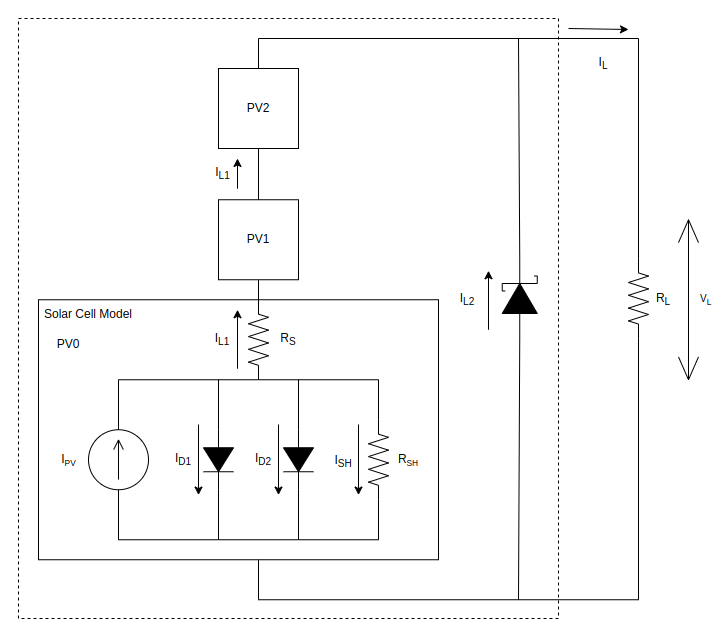
\includegraphics[width=\textwidth]{solar_module_model.png}
    \caption{Solar Module Model}
    \label{fig:solar_module_model}
\end{figure}

\subsection{Modeling Bypass Diodes}\label{subsec:bypass_diodes}

\subsection{Evaluation of Solar Module Models}\label{subsec:eval_solar_module_models}

\subsubsection{Solar Module Dataset}\label{subsubsec:solar_module_dataset}

\todo[inline,caption={}]{
    \begin{enumerate}
        \item Discussion of modules assembled, individual cell \ac{I-V} curves
        \item Discussion of lamination process (add reference to appendix for
        full procedure) and expected effect on efficiency
        \item
    \end{enumerate}
}

\subsubsection{Solar Module Test Setup}\label{subsubsec:solar_module_test_setup}

\todo[inline]{Refer to cell test setup and modifications for solar modules}


\subsubsection{Modeling Solar Module Datasets}\label{subsubsec:modeling_solar_module_datasets}

\todo[inline]{
    Compare Python model using extracted parameters against module \ac{I-V}
    curves.
}


\subsubsection{Evaluation of Solar Module Model}\label{subsubsec:evaluation_of_solar_module_model}

\todo[inline]{
    Holistic evaluation w/ table on statistics of model: e.g. for the model and
    extracted module parameters, what is the overall module accuracy and
    precision?
}

